\documentclass[british, svgnames, dvipsnames]{upb-beamer}
\usepackage[export]{adjustbox}
\usepackage[justification=centering, font=normalsize, labelfont={normalsize,bf}]{caption}
\usepackage{mathtools, amssymb, bm}
\usepackage{booktabs}
\usepackage{multirow}
\usepackage{subcaption}
\usepackage[style=american]{csquotes}

\setbeamertemplate{caption}[numbered]
\newcommand{\stimes}{{\times}} % No spaces \times operator


% --------------------------------------------------- %
%                  Presentation info	              %
% --------------------------------------------------- %

\title[Linear Image Filtering using HLS]{\textbf{\huge{Linear Image Filtering using HLS}}}
\author[Cristian Cristea]{\large{Reconfigurable Computing Project\\[0.5cm]\textbf{Cristian Cristea}}}
\institute[UNSTPB -- ETTI]{\small{Faculty of Electronics, Telecommunications and Information Technology\\[0.5mm]National University of Science and Technology POLITEHNICA Bucharest}}
\date{June 2024}

\setbeamersize{text margin left=5mm,text margin right=5mm} 

\graphicspath{{img/}}

% --------------------------------------------------- %
%                    Title + Schedule                 %
% --------------------------------------------------- %

\begin{document}

\begin{frame}
    \titlepage
    \makebox[0.91\paperwidth]{
        \centering
        
\includegraphics[width=1.4cm,keepaspectratio]{upb.eps}
        \hfill
        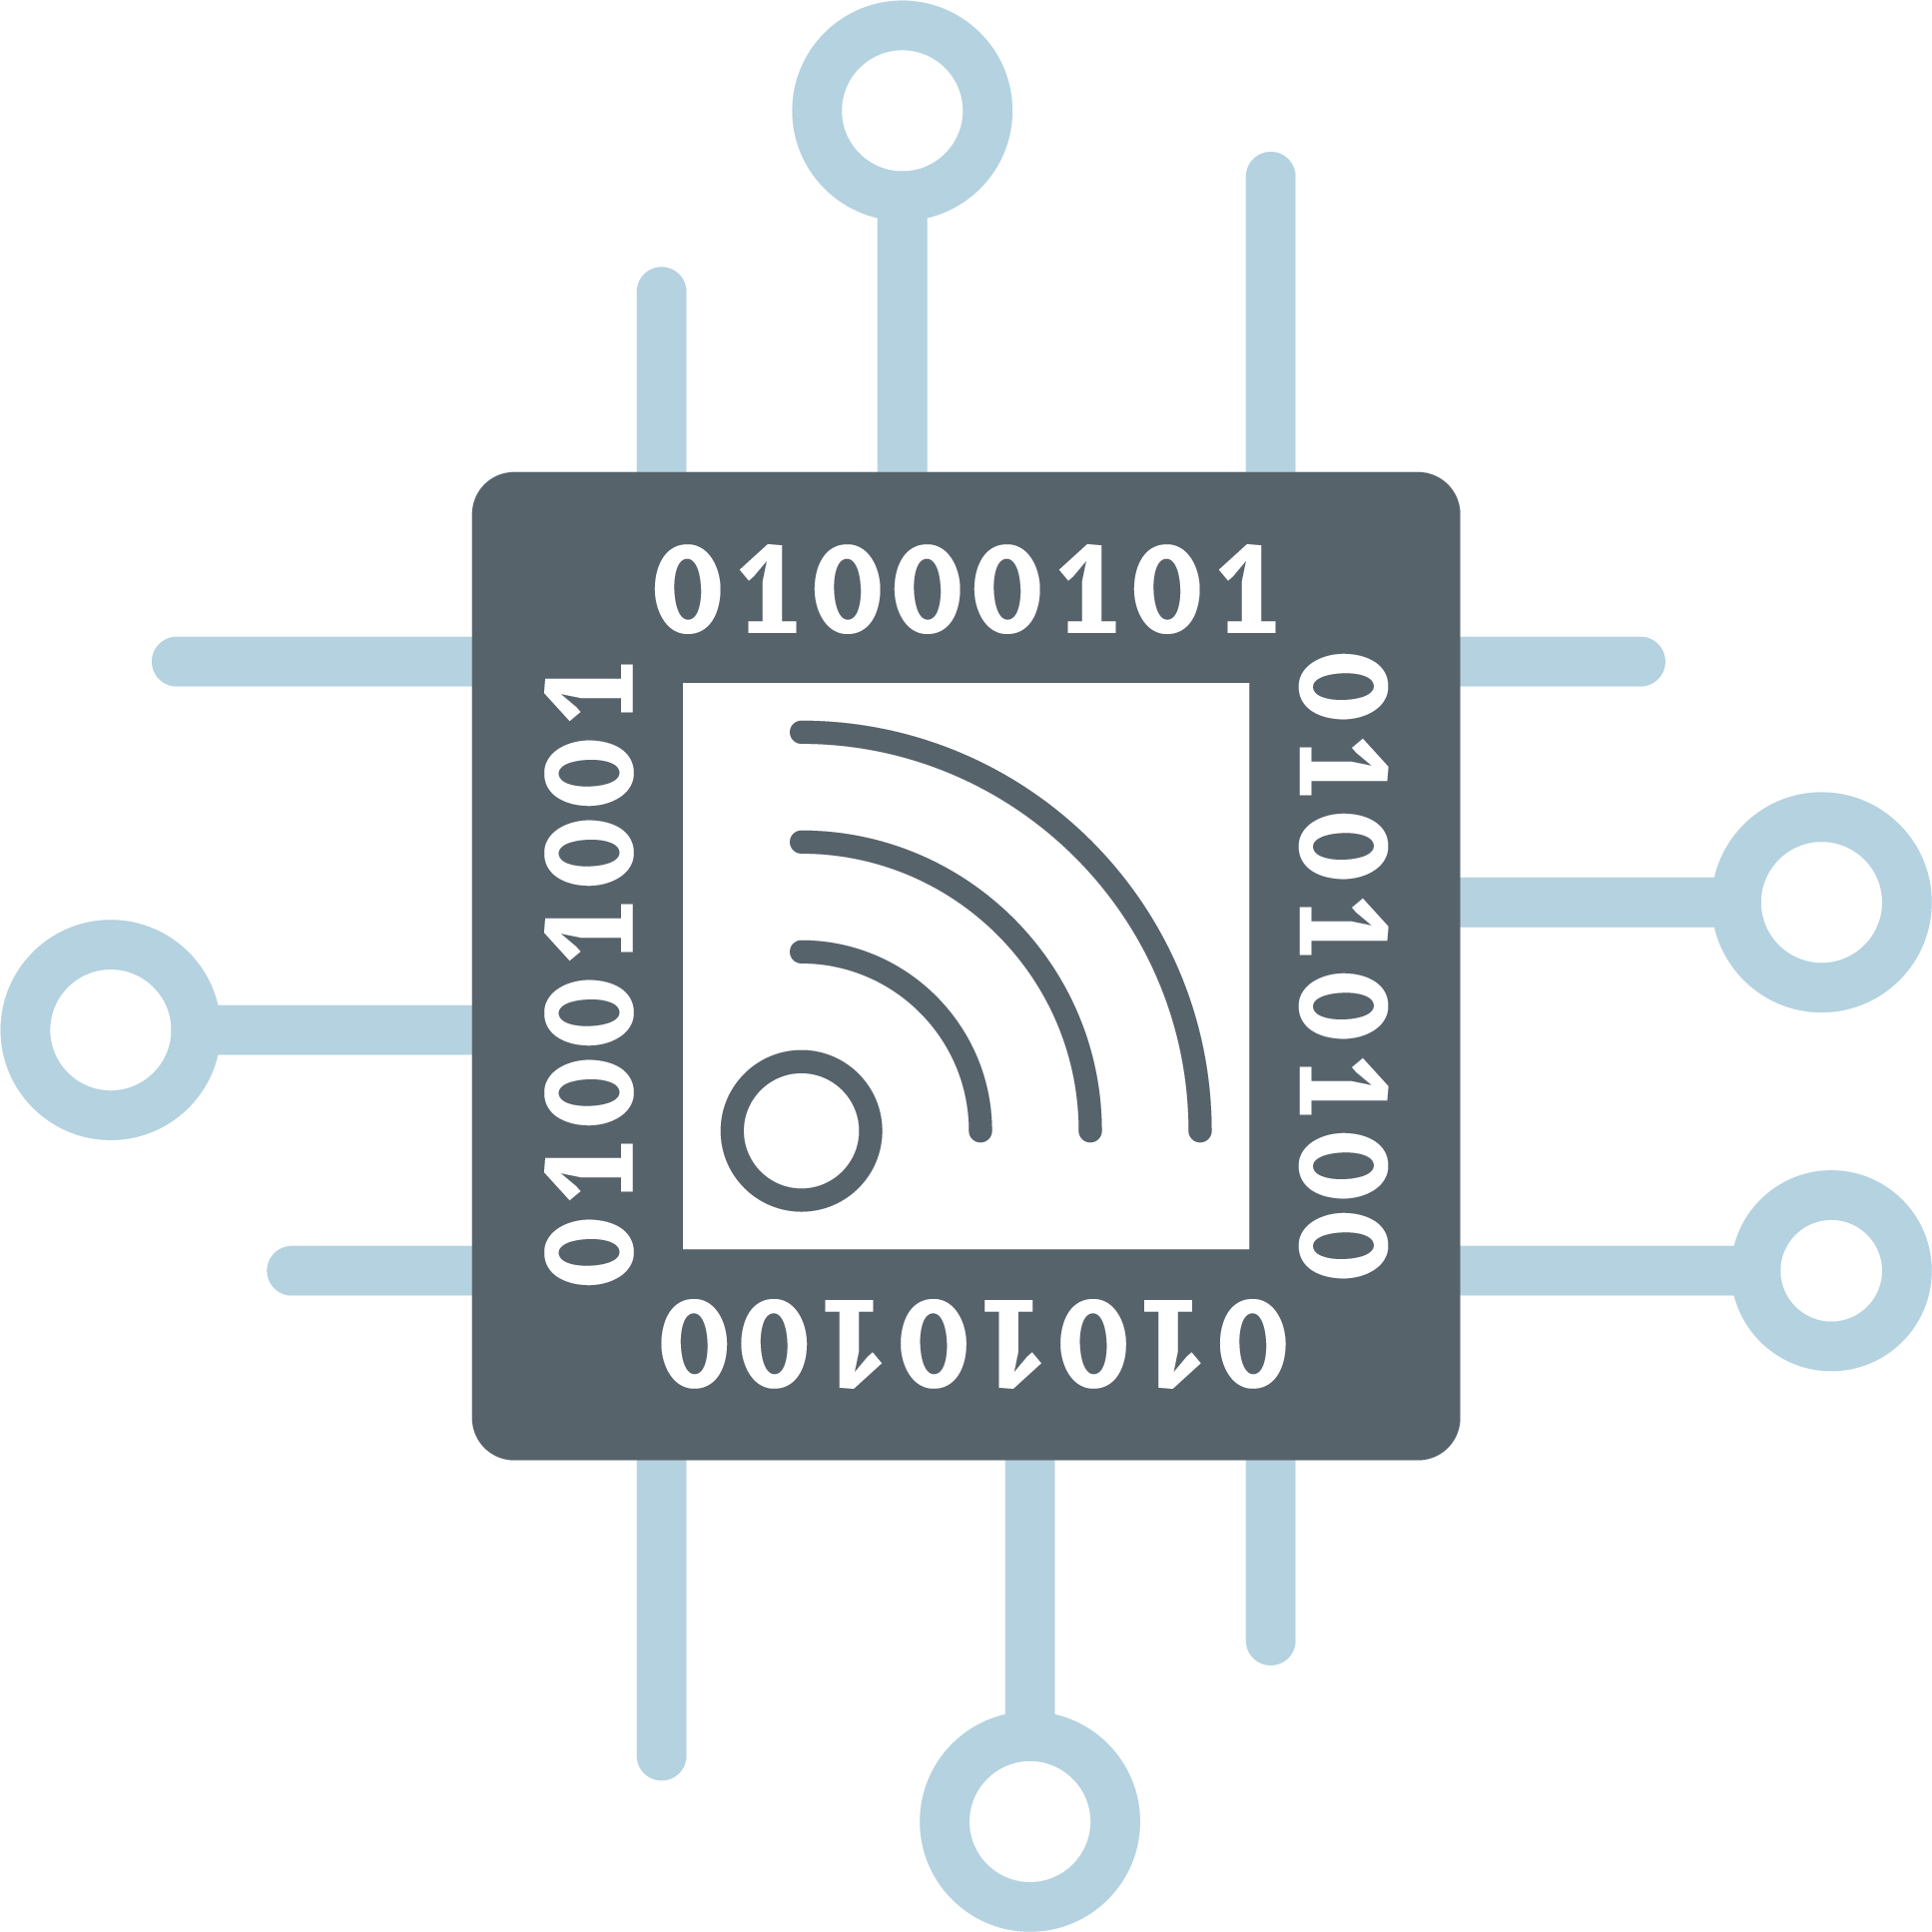
\includegraphics[width=1.4cm,keepaspectratio]{etti.png}%
    }%
\end{frame}

\begin{frame}{Table of Contents}
    \large{\tableofcontents}
\end{frame}

% --------------------------------------------------- %
%                    Presentation                     %
% --------------------------------------------------- %

% =================================================== %
\section{General Information}
% =================================================== %

\begin{frame}{Linear Image Filtering (Convolution)}
    \begin{columns}
        \begin{column}{0.5\textwidth}
            \begin{figure}[h!]
                \centering
                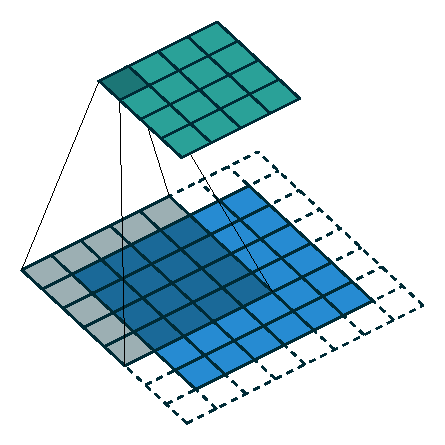
\includegraphics[width=\linewidth]{img/conv.pdf}
                \caption{Convolution with a $5\stimes5$ kernel (filter)}
                \label{fig:conv}
            \end{figure}
        \end{column}
        \begin{column}{0.5\textwidth}
            \begin{block}{Padding Methods}
                \begin{itemize}
                    \setlength\itemsep{0.5cm}
                    \item \textbf{Zeros} -- Adds rows and columns of zeros around the input image, preserving the spatial dimensions during convolution.
                    \item \textbf{Edge} -- Pads the input with the edge values of the image, replicating the border elements.
                    \item \textbf{Reflect} -- Extends the input by reflecting the values at the boundaries, creating a mirror effect.
                \end{itemize}
            \end{block}
        \end{column}
    \end{columns}
\end{frame}

\begin{frame}{Mean Filtering}
    \begin{center}
    \Large
        \[
        \bm{K} \vcentcolon= \dfrac{1}{n^2}\begin{bmatrix}
                    1 & 1 &\dots  & 1\\
                    1 & 1 &\dots  & 1\\
                    \vdots & \vdots & \ddots & \vdots\\
                    1 & 1 &\dots  & 1
                 \end{bmatrix}_{n\times n}\,, n\bmod2\equiv1.
        \]
    \end{center}
\end{frame}

\begin{frame}{Mean Filtering}
    \begin{figure}[h!]
        \centering
        \captionsetup[subfigure]{justification=centering}
        \begin{subfigure}[b]{0.49\textwidth}
            \centering
            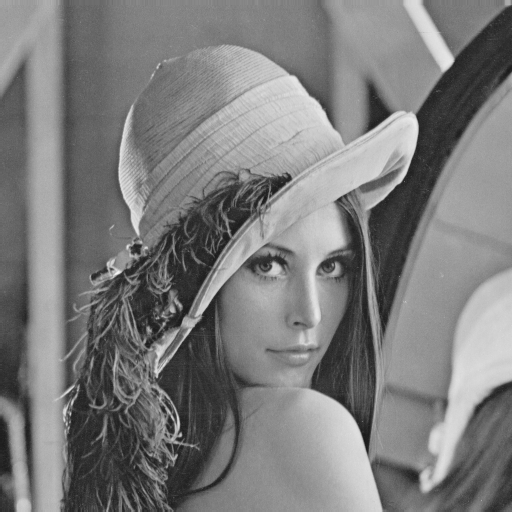
\includegraphics[width=\linewidth]{img/original.png}
            \caption{Original black and white Lena picture}
            \label{fig:original}
        \end{subfigure}
        \begin{subfigure}[b]{0.49\textwidth}
            \centering
            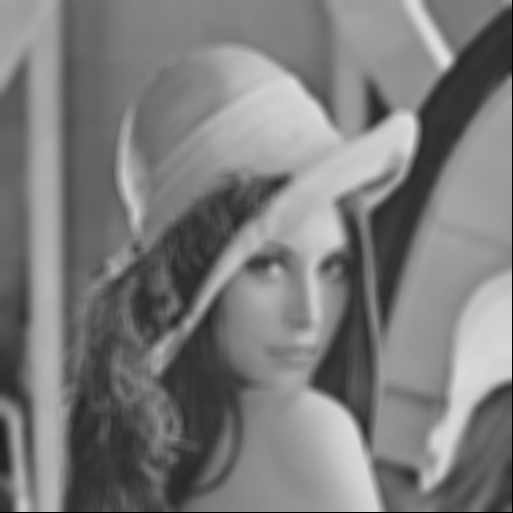
\includegraphics[width=\linewidth]{img/filtered.png}
            \caption{Filtered with a $11\stimes11$ mean kernel}
            \label{fig:filtered}
        \end{subfigure}
        \caption{Input and output of a convolution}
        \label{fig:avrs}
    \end{figure}
\end{frame}

% =================================================== %
\section{Progress}
% =================================================== %

\begin{frame}{Optimisation Changelog}
    \begin{itemize}
        \setlength\itemsep{0.5cm}
        \pause
        \item \textbf{Version 1} -- Initial implementation of the project by transforming the reference C++ code into a Vitis project.
        \pause
        \item \textbf{Version 2} -- Implement caching for the input image and the kernel matrix in BRAM memory to reduce the memory access time.
        \pause
        \item \textbf{Version 3} -- Unroll the columns loop in the image processing loops to increase the parallelism of the algorithm.
        \pause
        \item \textbf{Version 4} -- Change the unroll to the rows loop in the image processing loops.
        \pause
        \item \textbf{Version 5} -- Change the input image cache to have shorter lines and more of them, reduce the unroll factor, and pipeline the padding function instead of inlining it.
        \pause
        \item \textbf{Version 6} -- Change the data type from \texttt{float} to \texttt{uint8\_t}, inline the padding function, remove the loop unrolling, and reduce the number of cache lines.
    \end{itemize}
\end{frame}

% =================================================== %
\section{Results}
% =================================================== %

\newcommand{\size}[1]{\textbf{$\text{#1}\times\text{#1}$}}

\begin{frame}{Results}
    \begin{table}[h]
    \resizebox{0.9\textwidth}{!}{%
    \begin{tabular}{lrrrrr}
    \toprule
     \textbf{Implementation} & \size{3} & \size{5} & \size{7} & \size{9} & \size{11} \\
     \midrule
     Reference on PC\footnote{Intel® Core™ i5-6600K (4 Cores, 4 Threads, 3.5 GHz - 3.9 GHz, 6 MB Cache)} & 491 ms & 1 083 ms & 1 974 ms & 3 154 ms & 4 594 ms \\
     Reference on Laptop\footnote{Intel® Core™ i7-9750H (6 Cores, 12 Threads, 2.6 GHz - 4.5 GHz, 12 MB Cache)} & 376 ms & 696 ms & 1 793 ms & 2 919 ms & 4 050 ms \\
     Reference on RPI 5\footnote{Broadcom BCM2712 - ARM® Cortex-A76 (4 Cores, 4 Threads, 2.4 GHz)} & 380 ms & 1 013 ms & 1 978 ms & 3 146 ms & 4 993 ms \\
     Reference on PYNQ-Z2\footnote{Xilinx Zynq-7000 - ARM® Cortex-A9 (2 Cores, 2 Threads, 0.65 GHz)} & 7 744 ms & 19 930 ms & 39 428 ms & 63 288 ms & 93 335 ms \\
     Version 1 on PYNQ-Z2 & 29 158 ms & 61 238 ms & 109 352 ms & 173 334 ms & 252 413 ms \\
     Version 2 on PYNQ-Z2 & 14 131 ms & 22 194 ms & 34 288 ms & 50 413 ms & 70 568 ms \\
     Version 3 on PYNQ-Z2 & 13 830 ms & 21 892 ms & 33 987 ms & 50 112 ms & 70 266 ms \\
     Version 4 on PYNQ-Z2 & 14 132 ms & 22 195 ms & 34 288 ms & 50 412 ms & 70 568 ms \\
     Version 5 on PYNQ-Z2 & 14 204 ms & 22 266 ms & 34 359 ms & 50 859 ms & 71 398 ms \\
     Version 6 on PYNQ-Z2 & 10 693 ms & 12 450 ms & 15 019 ms & 18 378 ms & 22 550 ms \\
     \bottomrule
    \end{tabular}
    }
    \caption{Results comparison for different kernel sizes}
    \label{tab:ref}
    \end{table}
\end{frame}

\begin{frame}{Conclusions}
    \begin{itemize}
        \setlength\itemsep{0.5cm}
        \pause
        \item The FPGA High-Level Synthesis (HLS) designs exhibited subpar performance compared to implementations executed on a PC, Laptop, and Raspberry Pi 5.
        \pause
        \item Implementing caching within the FPGA HLS designs significantly improved performance by reducing memory access times.
        \pause
        \item Optimisation techniques such as loop unrolling and pipelining did not decrease execution times.
        \pause
        \item A substantial increase in performance was achieved by changing the data type from floating point to integer-based.
        \pause
        \item Among the FPGA HLS designs, all except the one without caching outperformed the reference implementation running on the ARM core of the PYNQ-Z2 when large kernel sizes were employed.
        \pause
        \item Further analysis is needed to evaluate performance in the context of power consumption.
    \end{itemize}
\end{frame}

\begin{frame}
    \hfill\Huge{Thank you for your attention! Questions?}
    \color{structure.fg!75!black}{\rule{\textwidth}{0.05cm}}
\end{frame}

\end{document}
